\documentclass{article}
\usepackage[utf8]{inputenc}
\usepackage[a4paper, total={6in, 8in}]{geometry}

\usepackage{svg}
\usepackage{amsmath}
\usepackage{amssymb}
\usepackage{hyperref}
\usepackage{cleveref}
\usepackage{subcaption}
\usepackage[super]{natbib}

\title{Quantifying Uncertainty in Reconstructed Interferometric Images for the DSA-2000}
\author{Tyrone McNichols\\ Mentors: Katherine L.\ Bouman, Oscar Leong, Liam Connor}
\date{}

\begin{document}

\maketitle


\section{Abstract}
The DSA-2000 is a powerful upcoming radio interferometer that plans to use a feed-forward convolutional neural network called POLISH to reconstruct images from observed data. However, this process is ill-posed, meaning that there are several possible reconstructions that match the data. Moreover, these different reconstructions can have drastically different scientific interpretations, establishing a need for a measure of reliability in images. Here, we combine POLISH with the principles of Bayesian learning to allow the network to output a pixel-wise uncertainty estimate in addition to the reconstruction. This uncertainty estimate captures confidence in reconstructions as well as imperfections in the data set and model itself. We demonstrate this model using simulated radio sky data. Our model is able to provide accurate reconstructions and metrics needed to assess the reliability of those outputs. 


\section{Introduction}

A major focus of recent research in computational imaging has been inverse problems, where an unknown image is reconstructed from a set of measurements \cite{POGGIO1987638}. Inverse problems have applications in many fields including signal processing, computer vision, medical imaging, and astronomy. Traditionally, inverse problems are solved by framing them as an optimization problem. This optimization usually involves minimizing a cost function consisting of a data-fitting term, which ensures the reconstruction matches the observed data, and a regularizer, which incentivizes the reconstruction to exhibit certain desired properties based on prior knowledge. An optimization problem must be solved for every reconstruction, making this process potentially computationally expensive. Additionally, inverse problems often have many possible solutions consistent with the data, making them ill-posed. Different solutions often have very different scientific interpretations. Thus, it is necessary to understand the reliability of a single solution to better guide scientific analysis of images.

In recent years, deep learning techniques have been applied to solve inverse problems, drastically transforming the landscape of the field \cite{ongie2020deep}. Such techniques perform well in terms of reconstruction quality while also bringing additional benefits. Because deep neural networks can be pre-trained on data and generalize well, there is no need to solve an optimization problem at evaluation time. New measurements can be given to the same network to produce reconstructions without additional training. This ``feed-forward'' model allows users to process images much faster than traditional approaches. 

Deep-learning techniques have also been used to address the reliability problem of inverse problems \cite{sun2020deep}. Bayesian neural networks (BNNs) offer a way to measure uncertainty in network outputs. BNNs differ from normal neural networks in that they learn a probability distribution over the network parameters rather than deterministic weights. On each forward pass through the network, new weights are sampled from the learned distribution, creating an implicit distribution over the network outputs. When given the same input multiple times, a BNN will produce slightly different results. By analyzing the variance of this distribution, the reliability of a reconstruction can be quantified.

Here we are concerned with the imaging pipeline for the 2000-element Deep Synoptic Array (DSA-2000), an ambitious upcoming radio interferometer \cite{hallinan2019dsa2000}. This interferometer will produce an unprecedented amount of data, requiring the real-time performance allotted by feed-forward neural networks. In response to this need, the DSA-2000 team developed a convolutional neural network (CNN) called POLISH \cite{connor2021deep}. Currently, POLISH is capable of producing high-quality, super-resolved images, however reliability measurement remains an open problem for the pipeline. In this work, we address the reliability problem for POLISH. Following the work of \citet{Xue:19}, we adapt POLISH into a Bayesian neural network (BNN) that outputs a pixel-wise uncertainty estimate in addition to a reconstructed image. This framework allows us to quantify both the epistemic and aleatoric uncertainties in reconstructions, providing two descriptive measures for identifying low-confidence regions in images and analyzing potential sources of error.

\section{Methods}
In this section we describe our uncertainty learning framework. We first explain the mathematical basis for our method. We derive the loss function for our model, and provide methods to estimate both aleatoric and epistemic uncertainty. Next, we describe the network architecture for POLISH, and how it is adapted for our framework. Finally, we define the metrics we use to analyze performance.

\subsection{Types of Uncertainty}

In Bayesian modeling, there are two main types of uncertainty \cite{KIUREGHIAN2009105}. \textit{Aleatoric uncertainty} pertains to noise inherent in the observations. This uncertainty is caused by unknowns in the system that vary from measurement to measurement. This variance cannot be determined sufficiently in order to eliminate its influence, even with the observation of more data. Aleatoric uncertainty could be for example sensor noise. \textit{Epistemic uncertainty} on the other hand captures uncertainty in the model used to generate the observations. For a neural network, this is the uncertainty in the model's parameters. Unlike aleatoric uncertainty, epistemic uncertainty \textit{can} be explained away given enough data. Because large amounts of data are typically available in computational vision, it is often  effective to only model aleatoric uncertainty as it cannot be explained away. However, out-of-data examples can be identified with epistemic uncertainty, but not aleatoric uncertainty alone \cite{Kendall2017}. Therefore, it is essential that both uncertainties are modeled in our framework.


\subsection{Uncertainty Learning Framework}
\label{sec:uncert}
Our uncertainty learning framework relies on the probabilistic \textit{Bayesian neural network} (BNN). Unlike a standard neural network, a BNN learns a distribution over the network's parameters $w$.
Each time an input $x^\ast$ is 
given to the trained network, new weights are sampled from their respective 
distributions, resulting in a slightly different output $y$.
To quantify the variability of the output, we model  the \textit{predictive distribution} $p(y \mid x^\ast, X, Y)$ where $(X,Y) = \{x^i, y^i\}_{i=1}^N$ is the set of training data. This distribution is given through marginalization over all possible network weights:
\begin{equation}
    p(y \mid x^\ast, X, Y) = \int p(y \mid x^\ast, w)p(w \mid X, Y)\, \mathrm{d}w.
\end{equation}
The predictive distribution $p(y \mid x^\ast, w)$ describes all possible network outputs given the network weights $w$  and input image $x^\ast$. The posterior distribution $p(w \mid X, Y)$ describes all possible network weights given the training data.  We can evaluate the aleatoric and epistemic uncertainties by modeling $p(y \mid x^\ast, w)$ and $p(w \mid X, Y)$ respectively.

We employ the framework presented in \citet{Kendall2017} for designing BNNs that provide both 
aleatoric and epistemic uncertainty. We first modify the structure of POLISH to output two predictions: a predictive mean $\mu$ and a predictive scale $b$. To capture the \textit{aleatoric} uncertainty, we describe the probability distribution of the random output of the network with a Laplace likelihood function:
\begin{equation}
\label{eq:laplace}
        p(y_i \mid x, w) = \frac{1}{2b_i}\exp \left(  - \frac{| y_i - \mu_i|}{b_i}  \right),
\end{equation}
where the output pixels (denoted $i$) are assumed independent.
The negative log-likelihood of this distribution provides the minimization objective for training:
\begin{equation}
    \mathcal{L}_{\text{BNN}}(w\mid x, y) = \frac{1}{N}\sum_{i}\left(\frac{| y_i - \mu_i|}{b_i} + \log (2b_i)\right),
    \label{eq:loss}
\end{equation}
where $N$ is the number of pixels in the image. In practice, using \Cref{eq:loss} can result in numerical issues potentially dividing by zero. To circumvent this, the network instead predicts the
log predictive scale $s_i = \log (b_i)$, changing the loss function to:
\begin{equation}
    \mathcal{L}_{\text{BNN}}(w\mid x, y) = \frac{1}{N}\sum_{i}\left(|y_i - \mu_i|\exp(-s_i) + s_i \right).
    \label{eq:loss_log}
\end{equation}
This loss consists of two terms: a residual term resembling the L1 loss normalized by the standard deviation, and an uncertainty regularization term. The uncertainty regularization term prevents the network from simply outputting infinite uncertainty at all pixels. Notably, this loss function does not require a ground-truth scale value; the predictive scale $b$ is learned
implicitly from the loss function.
We then quantify the aleatoric
uncertainty $\sigma^{(A)}$ by computing the variance of the network outputs. Since we assumed a Laplace distribution over the network outputs in Equation  \ref{eq:laplace}, this is simply the variance of said distribution:
\begin{equation}
    \sigma^{(A)}_i = 2b^2_i.
\end{equation}

We model the posterior distribution $p(w \mid X, Y)$ using Monte Carlo dropout \cite{gal2016dropout}. By placing dropout after each weight layer during both training and evaluation, a simple distribution $q(w)$ is learned approximating $p(w \mid X, Y)$. Using Monte Carlo integration, we can then approximate the predictive distribution with $T$ Monte Carlo samples from the network, randomly sampling the network weights from $q(w)$ each time, i.e. $w^{(t)} \sim q(w)$:
\begin{equation}
    p(y \mid x^\ast, X, Y) \approx \int p(y \mid x^\ast, w)q(w)\, \mathrm{d}w \approx \frac{1}{T}\sum_{t=1}^T p(y\mid x^\ast, w^{(t)}).
\end{equation}
The predicted mean $\hat{\mu_i}$ for pixel $i$ can be estimated as:
\begin{equation}
    \hat{\mu}_i = \mathbb{E}[y \mid x^\ast, X, Y] \approx \frac{1}{T} \sum_{t=1}^T \mathbb{E}[y\mid x^\ast, w^{(t)}] \approx \frac{1}{T}\sum_{t=1}^T \mu^{(t)}_i.
\end{equation}
Variations in this value are a direct consequence of uncertainty in the model parameters, thus capturing the \textit{epistemic} uncertainty. In other words, the epistemic uncertainty $\sigma^{(E)}$ is given by the variance of the predicted mean:
\begin{equation}
\label{eq:sig_e}
    \sigma^{(E)}_i \approx \frac{1}{T}\sum_{t=1}^T (\mu^{(t)}_i - \hat{\mu}_i)^2.
\end{equation}
Also note that in this Monte Carlo regime, the aleatoric uncertainty becomes:
\begin{equation}
\label{eq:sig_a}
    \sigma^{(A)}_i \approx \frac{1}{T}\sum_{t=1}^T 2(b^{(t)}_i)^2.
\end{equation}

\subsection{Network Architecture}

\begin{figure}
    \centering
    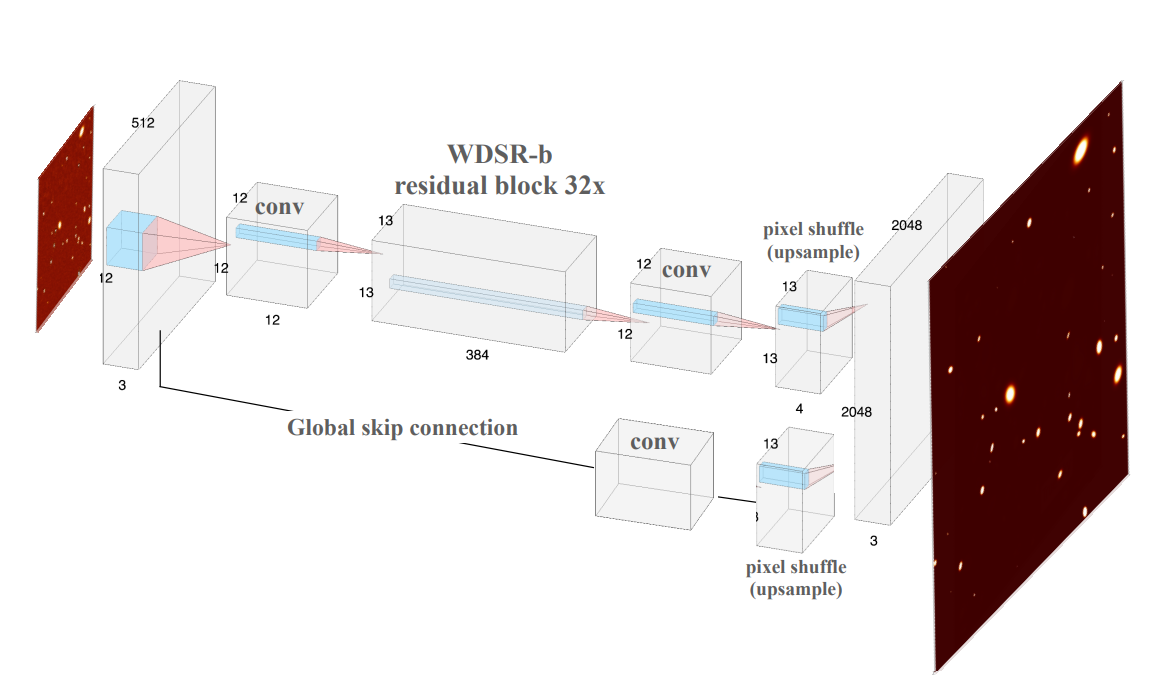
\includegraphics[width=0.8\linewidth]{img/POLISH.png}
    \caption{POLISH network architecture, adapted from \citet{Yu2018}. A dirty image is provided as input to the network, and the output is a deconvolved, super-resolved image.}
    \label{fig:polish}
\end{figure}


POLISH is a modified version of the Wide Activation for Efficient and Accurate Image Super-Resolution (WDSR) \cite{Yu2018} architecture. The WDSR architecture is a residual network based on a global skip connection and a ``residual block'' called WDSR\_b designed for efficient computation. The final layer of the network is a pixel shuffle, which upsamples the image by a factor of $s$. POLISH, takes as input a dirty image, $I_d$ with dimensions $(n_x, n_y, n_f)$ where $n_f$ is the number of frequency channels, and outputs a
super-resolved reconstruction of the sky, $\hat{I}_{\text{sky}}$, whose shape is $(sn_x, sn_y, n_f)$. \cite{connor2021deep}. A diagram showing the structure of POLISH is shown in Figure \ref{fig:polish}.

To adapt POLISH into a BNN, we add dropout layers after each convolutional layer in the network. This approximates the Deep Gaussian Process \cite{gal2016dropout}. Additionally, we modify POLISH to output an additional channel, the predictive scale $b$ for a total of $n_f + 1$ channels. The first $n_f$ channels of the output image correspond to the predicted mean $\mu$. We collect $T = 50$ Monte Carlo samples from the network to compute the two uncertainties given by Equations \ref{eq:sig_e} and \ref{eq:sig_a}.

\subsection{Performance Metrics}
We employ a number of metrics to analyze reconstruction quality. First we use peak signal-to-noise ratio (PSNR). This quantity estimates the ratio of maximum signal and corrupting noise in the image. Maximizing PSNR ensures that reconstructions will have little corruption, however it depends on pixel-wise error and so is sensitive to translations. To that end, we also use structural similarity index measure (SSIM), which compares windows in an image rather than absolute differences in pixels. It is also important to ensure that the same astronomical sources in the ground truth images are still present in reconstructions. SExtractor \cite{SExtractor} is a software package that detects sources in astronomical images and outputs catalogs with their positions and statistics. Using SExtractor, we extract a catalog of detected radio sources in both ground truth and reconstructed images, and compare the results. We produce a confusion matrix as a quantitative measure of catalog closeness. 

We also use two metrics for evaluating uncertainty predictions. First, we use calibration plots following the work of \citet{Kendall2017}. We compare the frequency of residuals falling within varying thresholds of the predicted distribution. We then plot this frequency vs the threshold value. For well calibrated uncertainty, this plot should closely match the line $y=x$. Additionally, we plot precision-recall curves to analyze how the model performs when removing pixels with uncertainty larger than certain thresholds.


\section{Results}


\subsection{Experimental Setup}

We test our method on synthetic astronomical data used for training POLISH. Our data is generated in the same fashion as in \citet{connor2021deep}, with true-sky images of size $1800\times1800$ pixels and an up-sampling factor $s$ of 3. For numerical stability, we further normalize training images to the range of $[-1, +1]$. These training images are made to accurately model what the DSA-2000 will actually observe. We train our model using 800 training image pairs for 1000000 training steps, and evaluate performance on a test set of 100 images. We implement our method in Tensorflow \cite{tensorflow2015-whitepaper}. In all experiments we use a dropout probability of $p=0.2$. We compare the results to the original POLISH as a baseline.


\subsection{Main Results}


\begin{figure}
    \centering
    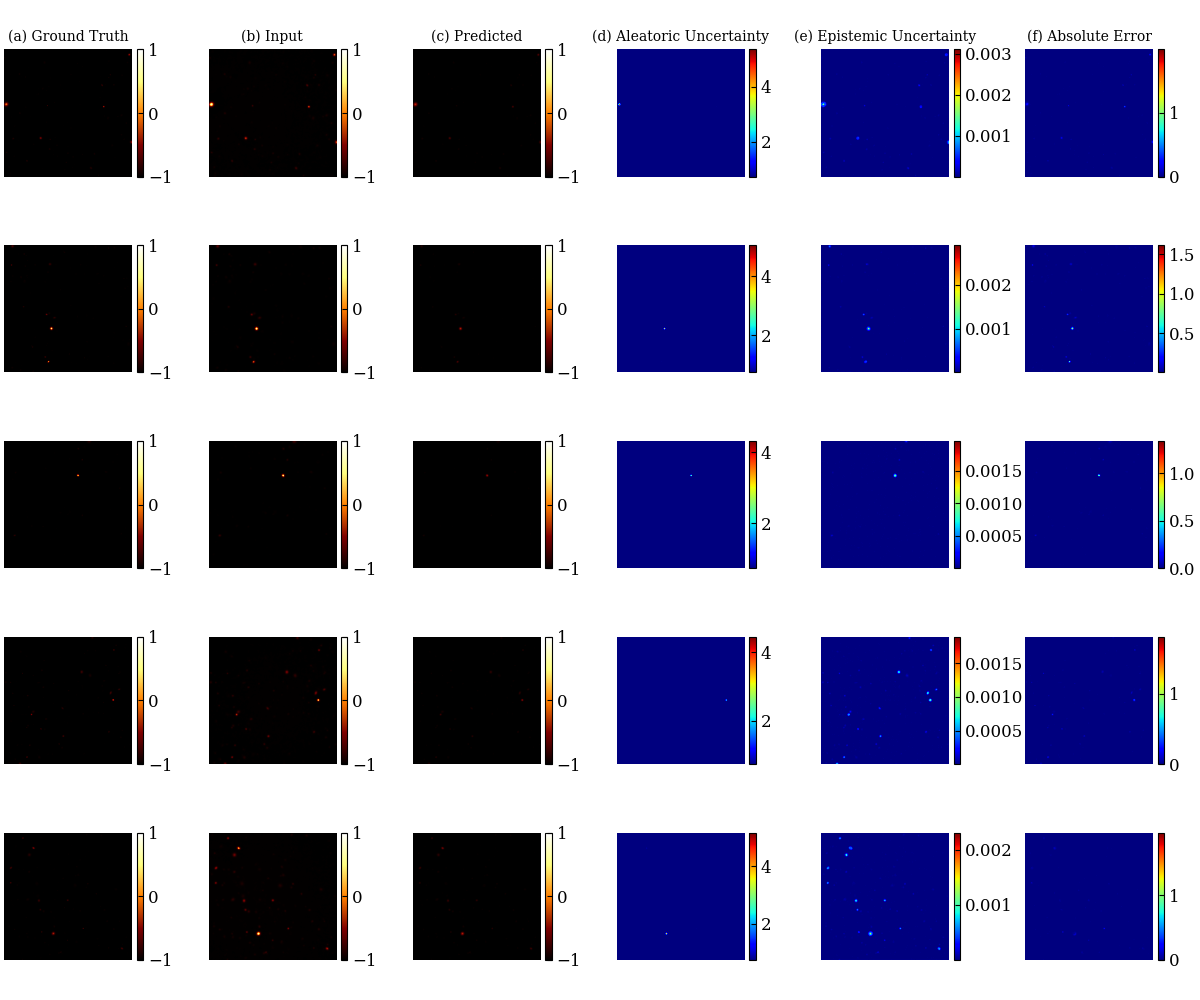
\includegraphics[width=\linewidth]{img/reconstructions.png}
    \caption{Sample reconstructions from POLISH BNN with uncertainty predictions. (a) The ground truth simulated image. (b) The dirty image which is given as input to the network. The BNN outputs (c) the mean prediction, (d) an aleatoric uncertainty estimate, and (e) an epistemic uncertainty estimate. (f) The absolute error between the ground truth and predicted mean.}
    \label{fig:examples}
\end{figure}

We demonstrate our method in Figure \ref{fig:examples}. Using our technique, POLISH is capable of outputting uncertainty estimates in addition to a reconstruction. Inspecting the uncertainty maps, we note that they correspond well with the absolute error. This shows that the uncertainty predictions can serve as an accurate indicator of possible reconstruction errors. We also note that the aleatoric uncertainty is much higher than the epistemic uncertainty. This suggests that error in our prediction is mostly from noise in the input data. The relatively small model uncertainty values further suggest that the BNN is capable of providing consistent results, as there is little variance in the actual reconstruction.

\begin{table}[]
    \centering
    \begin{tabular}{ccc}
        Metric & BNN (Our Method) & POLISH \\
         \hline
        PSNR & 46.542 & 49.614 \\
        SSIM & 0.9989 & 0.9994 \\
    \end{tabular}
    \caption{Comparison of reconstruction quality. We compare the average Peak signal-to-noise ration (PSNR) and structural similarity index measure (SSIM) for our method (left) and POLISH (right) on the test data set.}
    \label{tab:metrics}
\end{table}


\begin{figure}
    \centering
    \begin{subfigure}{0.3\linewidth}
        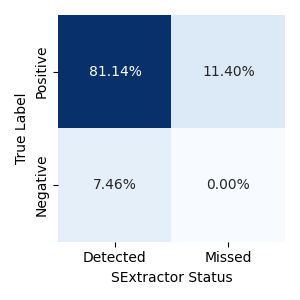
\includegraphics[width=\linewidth]{img/confusion.png}
        \caption{POLISH}
    \end{subfigure}
    \begin{subfigure}{0.3\linewidth}
        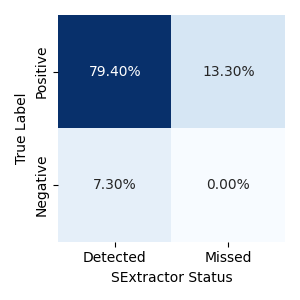
\includegraphics[width=\linewidth]{img/confusion_before.png}
        \caption{BNN}
    \end{subfigure}
    \caption{Comparison of confusion matrices. We compare the confusion matrices for source retrieval using SExtractor for both POLISH (left) and our BNN framework (right).}
    \label{fig:confuse}
\end{figure}

In Table \ref{tab:metrics}, we compare the PSNR and SSIM of our method to that of POLISH. Our method performs slightly worse, although the difference is negligible. We also compare confusion matrices for detected sources from SExtractor in Figure \ref{fig:confuse}.  We note that our model has a higher false-negative rate and a lower false-positive rate than POLISH. This may indicate that with the uncertainty estimate, our model learns to make more conservative predictions. Nonetheless, our model's performance is still comparable to the baseline. Together, these metrics show that our method is able to provide uncertainty estimates with minimal cost to reconstruction quality.


\subsection{Quantitative Analysis of Uncertainty Predictions}

\begin{figure}
    \centering
    \begin{subfigure}{0.45\linewidth}
        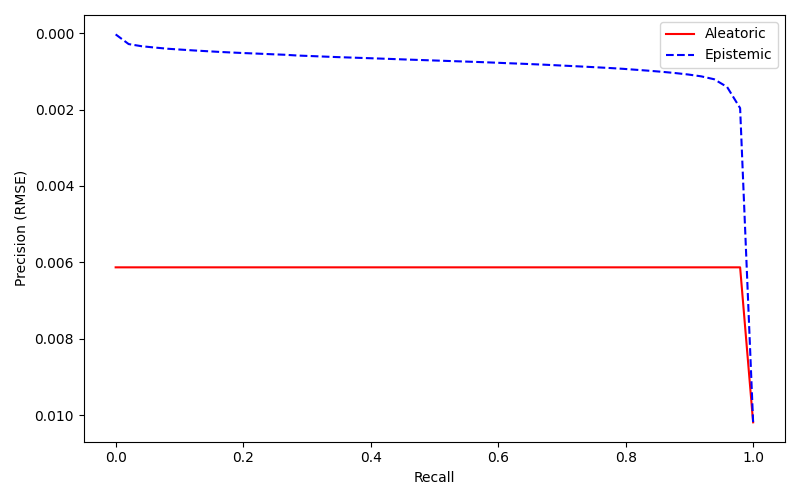
\includegraphics[width=\linewidth]{img/full_pvr_2.png}
        \caption{Precision vs Recall.}
        \label{fig:pvr}
    \end{subfigure}
    \begin{subfigure}{0.45\linewidth}
        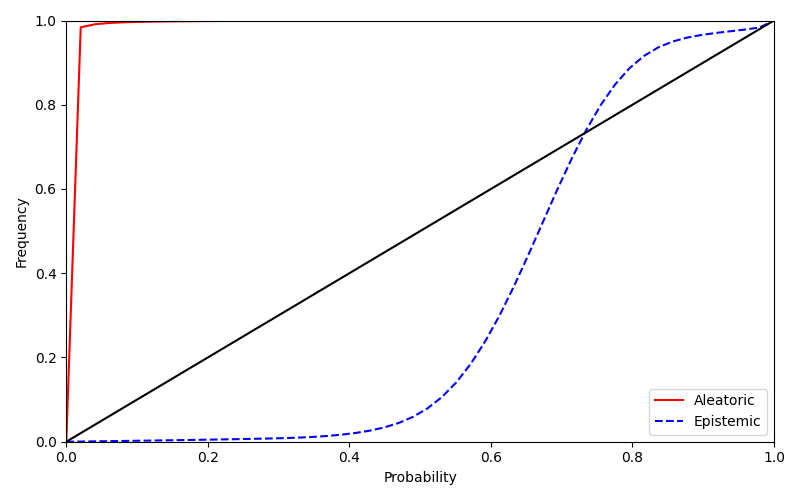
\includegraphics[width=\linewidth]{img/full_calibration_2.png}
        \caption{Calibration.}
        \label{fig:calibration}
    \end{subfigure}
    \caption{Quantitative plots for uncertainty prediction quality. On the left, we plot the precision vs recall. We compare the precision (y-axis, using RMSE) for varying percentiles of uncertainty. On the right, we demonstrates how well-calibrated the network is, where perfect calibration aligns with the line $y=x$.}
    \label{fig:uncert_anal}
\end{figure}

We plot the precision vs. recall curve for our method in Figure \ref{fig:pvr}. As the uncertainty increases the precision decreases, indicating that the measure is correctly correlated with accuracy. We note a steep decline in precision towards the end of the x-axis, where the pixels with the highest-uncertainty values are included in the measurement. This suggests that the pixels with higher uncertainty values are the ones deviating the furthest from the ground-truth image.

We also plot how well-calibrated network predictions are in Figure \ref{fig:calibration}. We note that the our model is quite poorly calibrated. The aleatoric uncertainty is far over-calibrated, that is it predicts higher uncertainty values than are accurate. Conversely, the epistemic uncertainty is under-calibrated for most of the data, although it much closer matches the ideal $y=x$ line.

\section{Conclusion}

We have presented an uncertainty-based learning framework for use with the DSA-2000. Our method produces high-quality, super-resolved images in a feed-forward fashion, which large radio interferometers like the DSA-2000 require for real-time image reconstruction. Furthermore, our method produces estimates of both the aleatoric and epistemic uncertainties, allowing researchers to assess reconstruction reliability. Our results indicate that these uncertainty estimates could provide a useful metric for identifying potential errors in reconstructions.

There are a couple of avenues left open for future work. First, further analysis of the uncertainty estimates is needed. In particular, we would like to compare the uncertainty map to the SExtractor source labels obtained. Ideally, false-positive and false-negative sources would correspond to higher uncertainty values than true-positives. Also, understanding the extent to which the two uncertainties are separated is important. Our model outputs aleatoric and epistemic estimates that are correlated with one another. However, the two uncertainties are expected to capture different errors. Additionally, working to produce uncertainty predictions that are better calibrated would improve confidence in the network outputs.

\section{Acknowledgements}

I thank my mentors Katie, Oscar, and Liam for their guidance and help. I'd also like to thank all the other members of Computational Cameras group for their feedback in developing this project. I also thank the SFP program for organizing and helping to fund this SURF. In particular, I thank Ms.\@ Betty Huang for providing financial assistance via the Associates SURF Fellowship. 




\bibliographystyle{unsrtnat}
\bibliography{ref}


\end{document}
